\documentclass{article}

\usepackage[inline]{enumitem}

\usepackage{url}
\usepackage{graphicx}
\graphicspath{ {./figures/} }
\usepackage{amsfonts}% to get the \mathbb alphabet
\usepackage{booktabs}
\usepackage{multirow}


\title{Decentralised Mining Pool for Bitcoin (Draft 0.1)}
\author{Kulpreet Singh}
\date{February 2021}

\begin{document}

\maketitle

\begin{abstract}
  Bitcoin p2pool's usage has steadily declined over the years,
  negatively impacting bitcoin's ability to remain decentralised. The
  primary problems with p2pool were twofold. First, the variance in
  earnings for miners didn't reduce with the increase in hashrate
  participating in p2pool. Secondly, payouts to miners required a
  linearly increasing blockspace with the increase in the number of
  miners on p2pool. Building a DAG of miner's shares and the use of
  payment channels are two proposals trying to alleviate these
  problems faced by p2pool. In this document, we present a unified
  solution that uses a directed acyclic graph to track miners shares
  and uses payments channels to reward miners. The shares calculation
  can be carried out by any node on the p2p network, and the rewards
  are paid out by a hub. Using the payment channels construction
  neither the hub nor the miners can cheat. We show that our approach
  is incentives compatible and reduces variance in earnings for
  miners. We also show how the hub increases its anonymity and avoids
  a DDoS attack on itself by using I2P to communicate with the miners.
\end{abstract}
   
\section{Motivation}

P2Pool~\cite{p2pool:wiki} helped in decentralising bitcoin by allowing
miners to select which transactions they mined and thus avoid any
potential transaction censorship by pool operators. However, the
construction used by P2Pool faced a number of problems that eventually
lead to miners abandoning the pool.

\begin{enumerate}
\item Large variance in earnings for miners.
\item Large number of dead on arrival blocks.
\item Large block space requirement.
\end{enumerate}

The first two problems are a direct consequence of the shares block
rate limited to 30 seconds. With only one block possible every thirty
seconds, any increase of hashrate on P2Pool resulted in shares
competing to be the next block in the p2pool chain. However, if the
pool wanted to increase the block rate frequency, it didn't increase
the throughput of the pool in terms of number of shares found, as most
of them are orphaned and the miners not being rewarded for those
orphans. Ethereum's inclusive protocols~\cite{inclusive-protocols}
help alleviate the problem for the Ethereum blockchain, where small
pools can work with a reduced variance in their rewards as shown in
the analysis by McElrath~\cite{mcelrath:variance}.

Knowing the challenges faced by P2Pool, we list the goals of a new
decentralised mining pool as:

\begin{enumerate}
\item Reduced variance for miners with increasing pool hash rate.
\item Independent miners that build their own blocks.
\item Payouts for miners with constant size block space requirement.
\item Provide building blocks for a hash rate futures market.
\end{enumerate}

\section{Current Proposals}

TerraHash Coin~\cite{mcelrath:variance}, Jute~\cite{jute}
and~\cite{spectre} are some of the attempts to use a DAG for faster
block times. However, these works focus on changing the consensus
layer of bitcoin itself. The ideas in these proposals allowed miners
to produce shares that have conflicting transactions and then apply
rules to find a set of transactions acceptable at various cuts of the
DAG.\@

Instead we propose to build a DAG of miner shares to enable faster
block times and using this DAG for calculating distribution of payouts
between miners. We then propose using payment channels as defined by
Belcher~\cite{channels-for-rewards} to avoid using block space for
making payouts to miners. Belcher's construction uses payment channels
between federated hubs to pay miners after a block has been
successfully mined. The payouts are made after a long enough period,
similar to the 100 blocks requirements for spending from coinbase
transactions. Miners register with hubs where bitcoin has been locked
in to open payment channels to miners. The construction shows how both
miners and hubs can't cheat and how the funders of the hub can earn a
reward for funding the payment channels.

The ideas of the Hash Rate Futures and Payment Channels for Rewards
Payouts together present a potential path for rebooting P2Pool. In the
rest of the paper we present a modified version of TerraHash Coin and
show how the various components work together.

\section{Decentralised Bitcoin Mining}

In this section we present a modified version of TerraHash Coin and
show how to build a DAG of miner's shares and use that to determine
the payout distribution between miners. We then show that the payout
distribution rewards miners for all the shares they find and
broadcast to the p2p network.

\subsection{A DAG of Shares}

The braiding the blockchain proposal~\cite{mcelrath:variance} shows
how smaller more frequent blocks can form a directed acyclic graph
(DAG) of blocks, with each block pointing to one or more one previous
blocks. Blocks in TerraHash Coin can have transactions repeated in
different blocks. The proposal describes how repeated and potentially
some double spend transactions can be resolved to decide on the state
of the ledger at any cut of the DAG.\@

The rewards that miners earn in the proposal is a coin native to the
braid blockchain and is called TerraHash Coin. This coin can then be
swapped for Bitcoin. The proposal doesn't yet define how this native
coin will be swapped by bitcoin. Some of the suggestions under
discussion include using atomic swaps, burning the TerraHash Coin, or
using financial instruments like futures of the bitcoin's hash rate to
swap TerraHash Coins for BTC.\@

We propose taking a modified approach, where the blocks of a DAG
represent shares of the mining pool. The DAG is maintained by each
participant in the p2p network as a replicated database. Shares
broadcast by miners include a hash pointer to all previous shares
received from other miners, this ensures the DAG is eventually
consistent on all p2p participants.

\subsubsection{Building Blocks}\label{sec:building-blocks}

Each miner builds their own block, selecting transactions according to
their own criteria. We call this block the \textsc{work}. The
description of \textsc{work} is then disseminated to the p2p network
of miners using the compact block
specifications~\cite{compact-blocks}.

The miner then starts mining on \textsc{work} and generates
\textsc{share}s. Each \textsc{share} is mined at a difficulty level
chosen by the miner. This difficulty can be dynamically chosen by the
miner after each \textsc{share}, depending on miner's observation of
the p2p network's hashrate. This dynamic adjustment allows miners to
adjust the rate at which they produce \textsc{share}s.

Figure~\ref{fig:work-share} shows the relationship between
\textsc{work} and its \textsc{share}s. Each \textsc{work} created by a
miner can result in multiple \textsc{share}s and both the
\textsc{work} and \textsc{share}s are broadcast to the p2p network.

\begin{figure}
  \begin{center}
    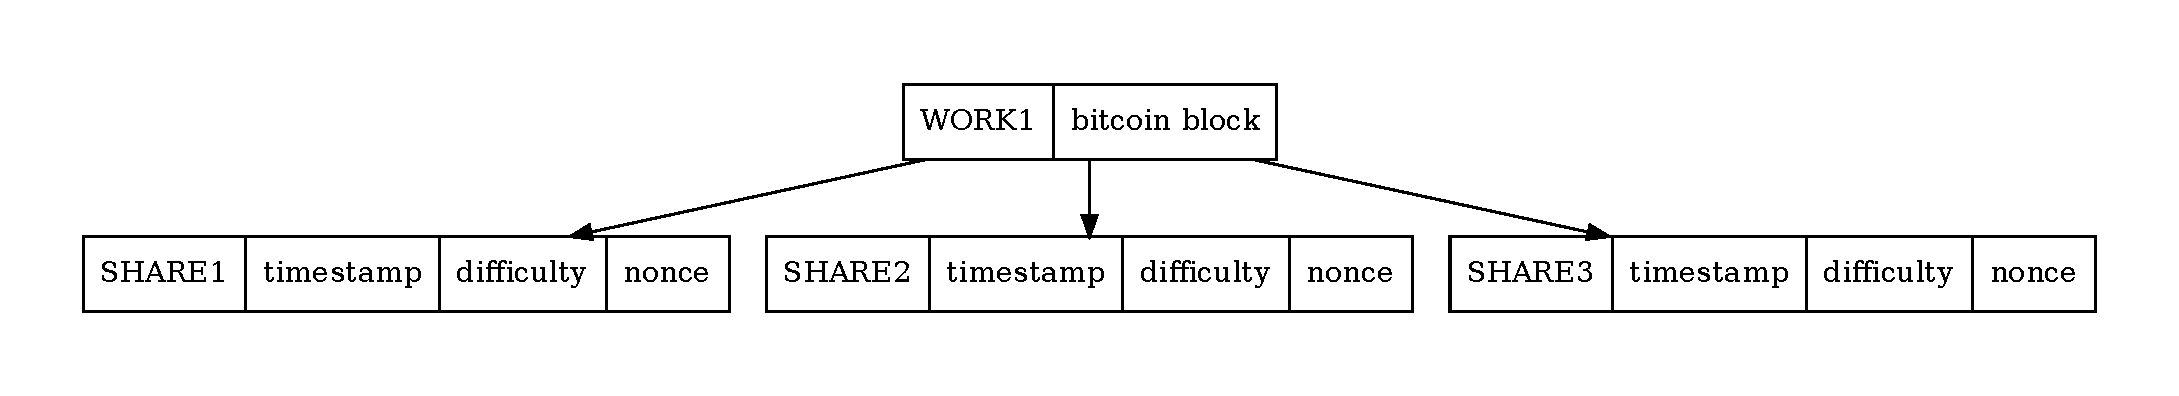
\includegraphics[width=1.0\textwidth]{work-share}
    \caption{Each \textsc{work} generated and shared by a miner is then
      followed by the \textsc{share}s the miner finds.}\label{fig:work-share}
    \end{center}
\end{figure}

The nodes in the DAG are \textsc{share}s mined at varied difficulty
levels. Each \textsc{share} that matches or exceeds the current
bitcoin difficulty starts a new $epoch$ for the p2p mining
pool. Figure~\ref{fig:epoch} shows $l$ and $r$ as the two valid
bitcoin blocks that have been mined such that they meet bitcoin's
difficulty at the time the block was mined, and all the blocks between
$l$ and $r$ are in the same $epoch$.

\begin{figure}
  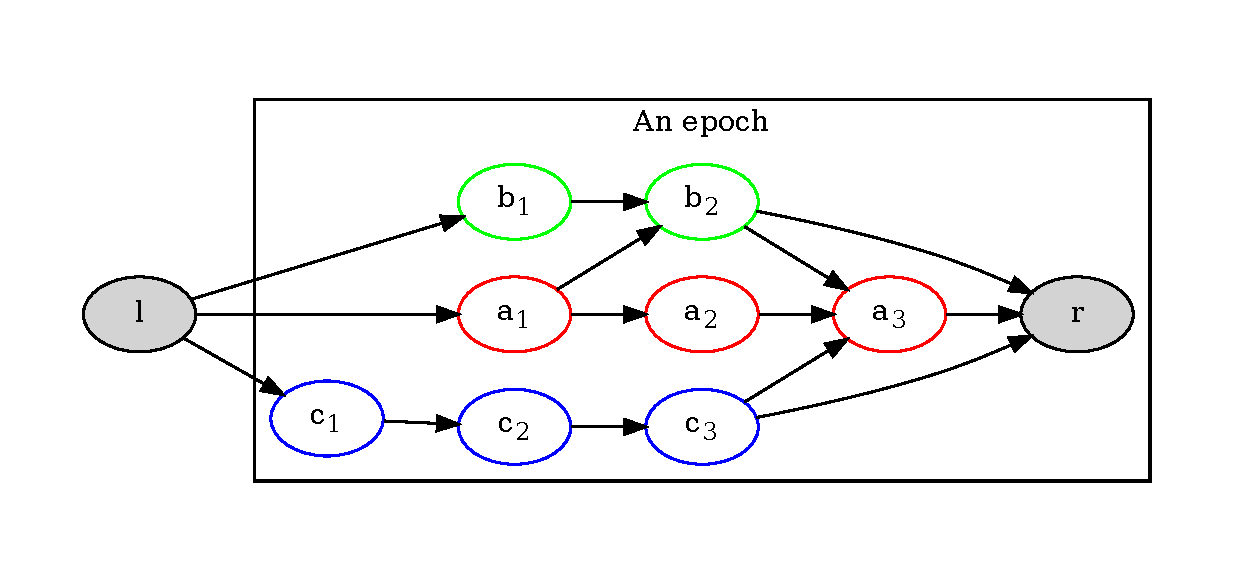
\includegraphics[width=1.0\textwidth]{epoch}
  \caption{A epoch is defined as all the \textsc{share}s mined between two
    bitcoin blocks. Here all the \textsc{share}s between $l$ and $r$ are in
    the same $epoch$.}\label{fig:epoch}
\end{figure}

When a miner starts working on a \textsc{share} it includes a
reference to the most recent \textsc{share} from all other miners that
the miner has received valid shares from. Note, the miner also has
access to \textsc{work} blocks from all participating miners. If a
miner doesn't have the \textsc{work} block from another miner, then it
rejects any \textsc{share}s received from the other miner.

In the next section we then describe how all peers compute their fair
share of profits using the DAG of shares. We then show how our reward
computation algorithm is incentives
compatible~\cite{incentives-compatible}.

%% - block datastructure
%%   - coinbase reward goes to Hub's address
%%   - ignore this for now, we'll show how the reward is distributed in a
%%     trustless manner to all miners.
%% - DAG of shares
%%   - Epochs: start from and end with bitcoin block
%%   - Epoch ends when a valid bitcoin block with current bitcoin
%%     difficulty is found
%%   - Immediately send mined bitcoin block to bitcoin network
%%   - Hub will distribute the reward in around 100 blocks time
%% - Use compact blocks to inform others about the block we are mining
%%   - Other miners can decide to include your block as a previous block
%%     or not, whenever we find a solution and announce it.
%%   - We need to model the network traffic and latency
%% - Keep mining the same block, until end of epoch
%%   - For each block mined, share the solution with p2p network
%%   - Only if the mined block meets the current bitcoin difficulty
  
  
\subsection{Incentives Compatible Rewards}\label{sec:rewards}

Each participating node, which includes the miners and the hub,
maintains a replica of the the \textsc{share}s DAG.\@ Each
\textsc{share} includes a reference to the blocks the miner was aware
of when the \textsc{share} was found. The reason for doing so is
simple. If a miner $a$ doesn't include the \textsc{share}s of miner
$b$, then $b$ has a clear signal to stop including the \textsc{share}s
of $a$, and as we will see a miner wants that their \textsc{share}s
are referenced by other miners as only then they will be rewarded for
their work.

The incentive in lay terms is that all miners should honestly include
the \textsc{share}s discovered by other miners, as otherwise they will
most likely be excluded by other miners and they will lose the
opportunity to be rewarded for their work. We call this the
degenerative case of ``isolated miners'' and argue that miners have no
incentives to act in this manner. Figure~\ref{fig:isolated-miners}
shows a DAG where all three miners $a$, $b$ and $c$ are working
independently. In such a situation when the miner $a$ discovers a
share $a_3$ which is a valid bitcoin block but the reward is not
shared with any other miner.

\begin{figure}
  \begin{center}
    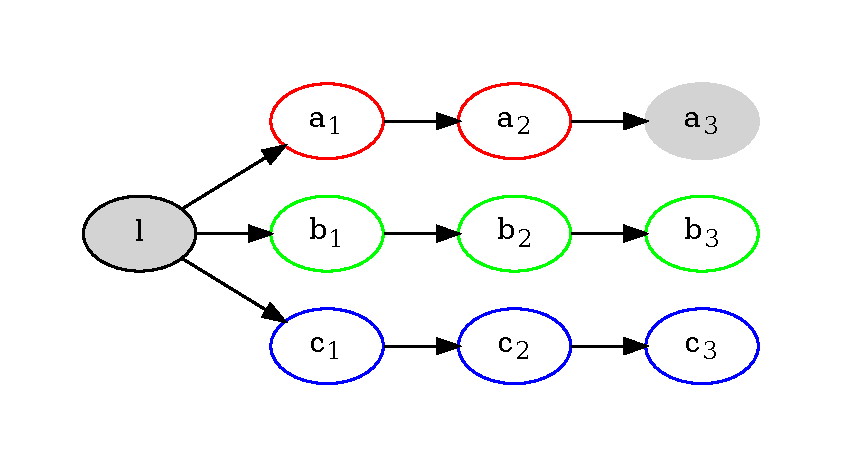
\includegraphics[width=0.5\textwidth]{isolated-miners}
    \caption{$a$ discovers a share and the reward is not shared with any
      other miner.}\label{fig:isolated-miners}
  \end{center}    
\end{figure}

With the above understanding of why miners will co-operate, we now
state the rules to calculate how the block reward should be divided
between miners.

\begin{enumerate}
\item Traverse the DAG in reverse order from the \textsc{share} that
  found a bitcoin block to the previous bitcoin block found and
  collect a set of shares.
\item From the above set of shares remove all shares that don't have
  a reverse path to the previous bitcoin block.
\item Distribute the reward between miners weighted by the sum of
  the difficultly of all \textsc{share}s found by miners.
\end{enumerate}

As an example consider the p2p network of miners $a$, $b$ and $c$ with
the DAG of shares as shown in Figure~\ref{fig:shares-dag}. In the DAG
the set of shares that receive reward proportional to their
difficulty are $\{a_i..a_5, b_1..b_3\}$. The shares $\{c_1..c_3\}$ do
not receive any reward as they are not reachable from the bitcoin
block, $a_5$, even if they are reachable from $l$.

For the second bitcoin block $b_5$ only the miners $a$ and $b$ receive
rewards in proportion to the difficulties of their shares
$\{b_4, b_5, a_6\}$. $c$ doesn't receive any reward for $c_4$ as it is
doesn't include a reference to the last found bitcoin block $a_5$.

\begin{figure}
  \begin{center}
    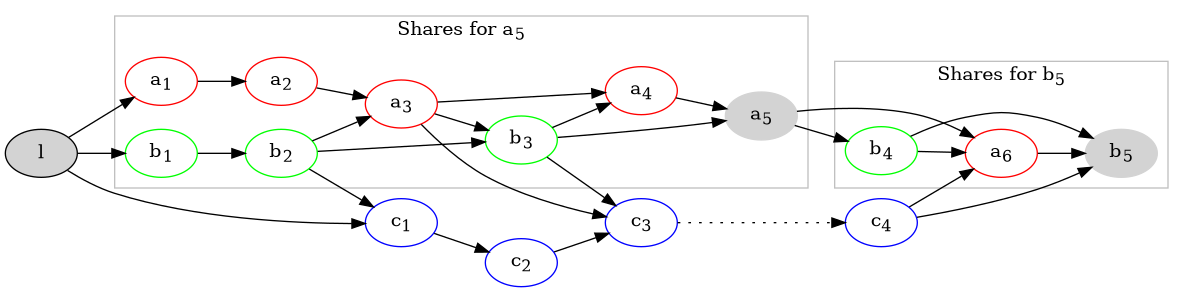
\includegraphics[width=1.0\textwidth]{shares-dag}
    \caption{Two epochs in a DAG of shares mined by three mines ---
      $a$, $b$ and $c$. The shares in grey meet the bitcoin difficulty
      at the time they were mined.}\label{fig:shares-dag}
  \end{center}
\end{figure}

Given the above rules, we show how they together provide an incentives
compatible reward function as defined
by~\cite{incentives-compatible}. We present an outline of proofs that
will be be formalised in future work.

\subsubsection{Incentive Compatibility}\label{sec:incentive-compatability}

A reward function is incentive compatible when every miner's best
response strategy reports full solutions
immediately~\cite{incentives-compatible}. Where a ``full solution'' is
a share that meets the bitcoin network's difficulty requirement.

Given the rules in Section~\ref{sec:rewards}, if a miner finds a
bitcoin block the miner wants to get maximum reward possible based on
all the shares it has found and therefore is incentivized to announce
their \textsc{share} as soon as they find it. The longer a miner
doesn't announce the bitcoin block to the bitcoin network, the higher
the probability that some other miner on the pool will find a
different bitcoin block. [TODO: I think we need to motivate with this
extra reward for the miner who finds the block, Belcher mentions it
too. This can be added to the rules/algorithm in the previous
section.]

\subsubsection{Proportional Payments}\label{sec:proportional-payments}

As per~\cite{incentives-compatible}, we require that miners are paid
in proportion to the amount of work they have performed.

Since rewards are calculated at the end of an epoch and a miner is
incentivized to include hash pointers to the most recent shares seen
from all miners, it directly follows that all miners are guaranteed
payments for their shares that have reached the miner who found the
block. It is also clear here that miners are incentivized to propagate
their shares to the network as fast as they can.

\subsubsection{Budget Balanced}\label{sec:budget-balanced}

Again, as per~\cite{incentives-compatible} we would like the pool
operator to never incur a deficit. From the rules, since rewards are
paid at the end of the epoch, a hub pays out rewards without losing or
retaining any amount.

\subsection{Payment Channels}\label{ref:channels}

We propose using Payment Channels for paying miners based on the work
by Belcher~\cite{channels-for-rewards}. The construction of the
payments channels we present is similar to Belcher's construction, but
there are a few changes and we highlight before describing the
details.

\begin{itemize}
\item We use the DAG based scheme to distribute rewards among miners,
  so we avoid the problem of estimating block rewards before miners
  have created their shares.
\item We use a single hub, and prevent DDoS attacks by keeping the hub
  hidden using I2P~\cite{i2p, i2p-censorship-resistance} for
  communication between the hub and miners.
\end{itemize}

% TODO
% Question: How do we know the Hub is not creating coinbases with
% different preimages with each miner?

% Answer: Miners receive the pubkey for all other miners with the
% \textsc{work} announcement. Using this and the structure of the
% coinbase transactions, miners validate that the coinbase matches the
% hub's preimage, and the miner's pubkey.

\subsubsection{Coinbase}

We use Belcher~\cite{channels-for-rewards} construction where each
miner builds a coinbase transaction that can be spent in one of the
following three ways:

\begin{enumerate}
\item Co-operatively by Hub and Miner, or
\item The Hub with a hash lock for pre-image \verb|X|, or
\item The Miner that found the bitcoin block, but after waiting
  for six months.
\end{enumerate}

The scriptPubKey for the above conditions in the coinbase can be
written as:

\begin{table}
  \centering
  \begin{tabular}{ l }
    \bfseries Coinbase \\
    \midrule
    \verb|2 H M 2 CHECKMULTISIG| \\
    \verb|OR| \\
    \verb|hash(X) + Hub P2WPKH| \\
    \verb|OR| \\
    \verb|M and CHECKSEQUENCEVERIFY 6 months| \\ 
    \midrule
  \end{tabular}
  \caption{Coinbase transaction with hub and miner public keys.}\label{table:coinbase}
\end{table}

These conditions mean that the hub can not spend the coinbase without
revealing the pre-image $X$. This pre-image is included in the
construction of payment channels, as we will see in the next
section. This use of pre-image in both the coinbase and the payment
channel definition guarantees that miners get paid for their
accumulated payouts if the Hub defects.

\subsubsection{One-way Channels}

One-Way payment channels between hub and all miners allow miners to
receive payouts without consuming any blockspace in the bitcoin block
they mined. The use of payment channels is what makes braidpool scale
up without losing blockspace. Braidpool thus avoids losing the fees
that can be earned from the blockspace.

Just like in the early versions of proposal by Belcher we use one-way
payment channels. One-Way payment channels solve the problem of
aggregating a miner's payouts requiring a single blockchain
transaction for spending multiple payouts earned from their PoW
shares.

We use one-way instead of 2-way payment channels as an initial
implementation for Braidpool. If required we can switch to 2-way
channels~\cite{poon2016bitcoin} allowing miners to spend their mining
payouts over the lightning network. However, for now, we deliberately
stay away from the complexity of making the hub a lightning node. If
there is interest from miners to use the lightning network, we can
build that out in future.

Each miner has a one-way payment channel with the hub using a two of
two multisig with a time lock of six months. For each payout a miner
receives over the payment channel, the hub will charge an agreed upon
fees between the miner and the hub. Belcher's proposal recommends a
$0.1\%$ fees for the hub.

\subsubsection{Transactions}

The hub creates a funding channel locking an amount $R$ of
bitcoin. The miner then creates a refund transaction, spending the
funding transaction and sending the $R$ bitcoin back to the Hub. The
refund transaction has a locktime of six months allowing the miner to
accumulate their payout over the six month period. The protocol can be
extended to allow each miner to agree upon a locktime with the
hub. The trade-off will be between the fees charged by the hub and the
length of the locktime.

The funding transaction includes an input from the hub and an output
that can be spent in one of the two conditions shown in
Table~\ref{fund-tx}. \verb|H| and \verb|M| are the public keys for Hub
and Miner, they are called the co-operative keys by Belcher. While
\verb|H'| and \verb|M'| are alternative public keys for Hub and Miner,
and are called the uncooperative keys in the Belcher proposal.


\begin{table}
  \centering
  \begin{tabular}{ ll }
    \multicolumn{2}{c}{\bfseries Fund Transaction} \\
    \midrule
    \bfseries Input & \bfseries Output \\
    \midrule
    Hub's UTXO & \verb|2 H  M  2 CHECKMULTISIG| \\
    (Signed by the hub) & \verb|OR| \\
                    & \verb|2 H' M' 2 CHECKMULTISIG + Hash(X)| \\
    & (R coins) \\
    \midrule
  \end{tabular}
  \caption{Fund transaction for payment channel between hub and miner.}\label{fund-tx}
\end{table}


The hub doesn't broadcast the funding transaction instead it waits for
the miner to create refund transaction. This is the same as any other
timelocked one-way channel construction, i.e.\ the Miner creates a
refund transaction with a timelock, signs it and sends it to the
hub. The refund transaction is show in Table~\ref{refund-tx}.

\begin{table}
  \centering
  \begin{tabular}{ ll }
    \multicolumn{2}{c}{\bfseries Refund Transaction. Locktime 6 months} \\
    \midrule
    \bfseries Input & \bfseries Output \\
    \midrule
    Fund Tx & \verb|P2WPKH Hub's address| \\
    (Signed by miner) & (R coins) \\
    \midrule
  \end{tabular}
  \caption{Refund transaction signed by miner and held by
    hub.}\label{refund-tx}
\end{table}

With the refund transaction, if the Miner stops responding, the Hub
can get a refund in six months time. However, the hub can be attacked
by sending requests to open new channels and locking up the hub's
liquidity. Hub responds to a miner's channel open request only after
the miner has contributed enough shares. The threshold number of
shares required before opening the channel is a configuration
parameter for the hub. The miner will still receive the payouts for
the shares generated, it is only that the channel opening is delayed.

On receiving the refund transaction, the hub broadcasts the funding
transaction. Once the funding transaction is confirmed, the hub can
start sending payouts to the miner. These payouts are determined in
proportion to the shares found by the miner and included in the DAG as
described in Section~\ref{sec:rewards}.

The payment transactions are updates to the channel where each update
increases the earnings of the miner. The payment transactions are
signed by the hub using the non-cooperating key, \verb|H'|. The
Table~\ref{payment-tx} shows the structure of the payment
transactions.

\begin{center}
  \begin{tabular}{ ll }
    \multicolumn{2}{c}{\bfseries Payment Transaction} \\
    \midrule
    \bfseries Input & \bfseries Output \\
    \midrule
    Fund Tx & \verb|2 H  M  2 CHECKMULTISIG| \\
    (Signed by the hub using H') & \verb|OR| \\
                    & \verb|2 H' M' 2 CHECKMULTISIG + Hash(X)| \\
                    & (Hub: $R - earnings$; Miner: $earnings$) \\
    \midrule
  \end{tabular}
\end{center}

The hub updates the payment channel for each miner with payouts as
determined by the incentives compatible rewards algorithm shown in
Section~\ref{sec:rewards}. In the next section we present how the
payouts are distributed, we then show how the hub and the miners are
disincentivized to cheat.

\subsection{Distributed Payout Algorithm}

Once a miner mines a share that also meets the currently bitcoin
difficulty, the miner immediately broadcasts the block to the bitcoin
network. The coinbase of this block as shown in
Table~\ref{table:coinbase} can now be spent by

\begin{description}
\item[Co-operative Branch:] The miner and the hub by both signing the
  first branch co-operatively.
\item[Hub Branch:] The hub alone, by publishing the pre-image \verb|X|.
\item[Miner Branch:] the miner alone, after waiting for six months.
\end{description}

The proposal by Belcher specifies a payout algorithm that requires the
hub updates the state of all channels, i.e.\ make payment to all
miners. Once it has done so, the miner signs the first branch of the
coinbase transaction and hands the coinbase to the hub. The hub can now
redeem the entire payout.

However, there is a small issue here about how the miner signing the
coinbase can know if the hub has updated the states of all payment
channels. One obvious solution might seem like the miner collects
acknowledgements from all other miners that they have received the
channel update. We still have to deal with the situation where the ACK
from some miners never arrives? Or worse still, if a miner purposely
doesn't send an ACK to stall the pool.

We propose that instead of requiring ACKs from all miners, we extend
the P2P protocol such that all miners store channel updates for all
miners and send them out again if required. This approach is similar
to the use of \emph{inv} and \emph{getdata} messages in bitcoin. We
elaborate further on this in
Section~\ref{sec:hub-miner-communication}, but for the purposes of
discussion we assume there is a mechanism that allows a miner to be
sure that the hub has updated the states of all payment channels.

% All miners also send heartbeat messages to hide hub as the source of
% traffic when a block is found. These are all end to end encrypted.

% These messages aren't part of the critical communication channel that
% broadcasts \textsc{work} and \textsc{share}, and is a much lower
% frequency communication.

% What if hub and successful miner collude to not pay anyone?

\subsection{Defecting Does Not Pay}\label{ref:defecting}

Using the above construction of the payment channel and the
distributed payout algorithm, we now show that defecting by the hub or
the miner doesn't pay.

\subsubsection{Hub Defects}\label{ref:hub-defects}

If the hub defects and pays itself from the coinbase it uses the
\verb|hash(X) + Hub P2WPKH| branch of the coinbase. In doing so, the
hub has to reveal the pre-image \verb|X|. With the pre-image
available, all miners can use the
\verb|2 H' M' CHECKMULTISIG + Hash(X)| branch of their payment channel
transactions and close their channels.

The hub could defect on the very first block mined and the miners
would lose all their earnings. But that will end the pool before it
could be useful.

The hub could defect after a few blocks have been mined. In such a
case the miners will receive their fair share of earnings for all
previous blocks, but it would again be the end of life for the pool.

Remember the hub charges fees to fund the payment channels between the
itself and the miners. When the pool ends, the hub loses a profit
making opportunity. We argue that the incentive to defect reduces as
the size of the pool grows.

\subsubsection{Miner Defects}\label{ref:miner-defects}

A miner that found the block could chose to not sign the co-operative
branch of the coinbase. In such a case, the hub will wait for a
timeout period much shorter than the locktime on the miner
branch. This will close all channels and require that all these
channels be opened again.

Such an attack by the miner will hurt miners on the network who have
not yet earned enough payouts to amortise the cost of closing the
channel. However, the miner also loses any payouts since the last
block was found by the pool. A malicious miner could provide a large
portion of the pool's hash rate and then refuse to sign the
co-operative branches, this way it will make the pool defunct, but it
will be an expensive attack. Probably only one the state can afford,
and the only response to such an attack would be for the miners and
the hub to go underground.

\subsubsection{Hub and Miner Collude}\label{ref:collusion}

The hub and the miner could collude where they co-operate to spend the
coinbase to themselves without requiring that the hub pays all other
miners as per the reward schedule. The motivation for the miner is
clear that it earns a big payout, however, such an action by the hub
will end the pool and a stream of future profits for the hub.

%% \subsubsection{Miner Sybil Attack}\label{ref:sybil-attack}

\subsubsection{DDoS on the Hub}\label{ref:ddos-attack}

The hub could be attacked using a distributed denial of service attack
making it unable to process requests to open new channels and to
distributed payouts to miners. Belcher in his proposal suggested the
use of multiple hubs as a defence against such an attack. The proposal
also points out that multiple hubs will reduce the liquidity required
to open channels with miners.

According to Belcher's proposal, multiple hubs available on the p2p
network will enable miners to open channels to all hubs and receive
payouts from all the hubs. The coinbase is split between hubs in a way
that if any hub defects, the other hubs can still spend the coinbase
and split the block reward between them. In this way all miners
receive appropriate payouts.

Creating a larger coinbase for multiple hubs scales if we can use
Taproot~\cite{bip340,bip341, bip342} once it is activated. The
solution uses staggered timeouts for hubs to spend the coinbase in
case of defecting or hubs under DDoS attacks. We believe this option
is worth exploring once Taproot is enabled and the pool will benefit
from multiple hubs. This will be even more useful as with the multiple
hubs construction, 

We propose a different solution that requires a single hub. The
advantage is a simpler channel construction and allow us to build the
mining pool without waiting for Taproot activation. The single hub
approach requires that all miners open I2P tunnels to gateways and
publish the gateway's address in the shares they broadcast on the p2p
network. The hub then can communicate with miners by opening new
tunnels and remaining anonymous.

\subsection{Hub Miner
  Communication}\label{sec:hub-miner-communication}

The hub and the miner need to exchange messages at the time of channel
creation as well updating the channel state when the hub makes a
payout to the miners. The channel management messages are exchanged
infrequently as compared to the \textsc{share}s broadcast messages and
don't have the same timeliness requirements as the shares
broadcasts. We propose adoption a solution that doesn't compromise on
the hub's anonymity and makes a trade-off with increased latency of
the channel management messages.

We use I2P's tunnels to allow the hub to operate anonymously and
without being easily singled out for a DDoS attack. There are two
types of control messages the channel creation messages when the miner
first joins the pool and the payout messages whenever a block is
found. I2P works by setting up separate inbound and outbound
tunnels. According to the I2P documentation~\cite{i2p-tech-intro}:

\begin{quote}
  A tunnel is a directed path through an explicitly selected list of
  routers. Layered encryption is used, so each of the routers can only
  decrypt a single layer. The decrypted information contains the IP of
  the next router, along with the encrypted information to be
  forwarded. Each tunnel has a starting point (the first router, also
  known as ``gateway'') and an end point. Messages can be sent only in
  one way. To send messages back, another tunnel is required.
\end{quote}

With the tunnels setup, miners include their I2P destination address
in their share headers. The hub participates in the shares broadcast
p2p network and identifies a new miner and has access to the
destination address. Once the miner has mined for a certain time
period, the hub contacts the miner and provides its own destination
address in the
message~\cite{i2p-streaming-library}. Figure~\ref{fig:new-miner-communication}
shows how the ``Miner A'' announces its I2P destination address,
enabling the hub to contact the miner for exchanging channel creation
messages.

To prevent the tunnel endpoint and gateway from seeing the messages
being exchanged, the hub and the miner use I2P's layered encryption,
called garlic routing~\cite{i2p-garlic-routing}. With the destination
addresses of both the new miner and the hub known to each other the
two can proceed to anonymously setup a payment channel as described in
Section~\ref{ref:channels}.

\begin{figure}
  \begin{center}
    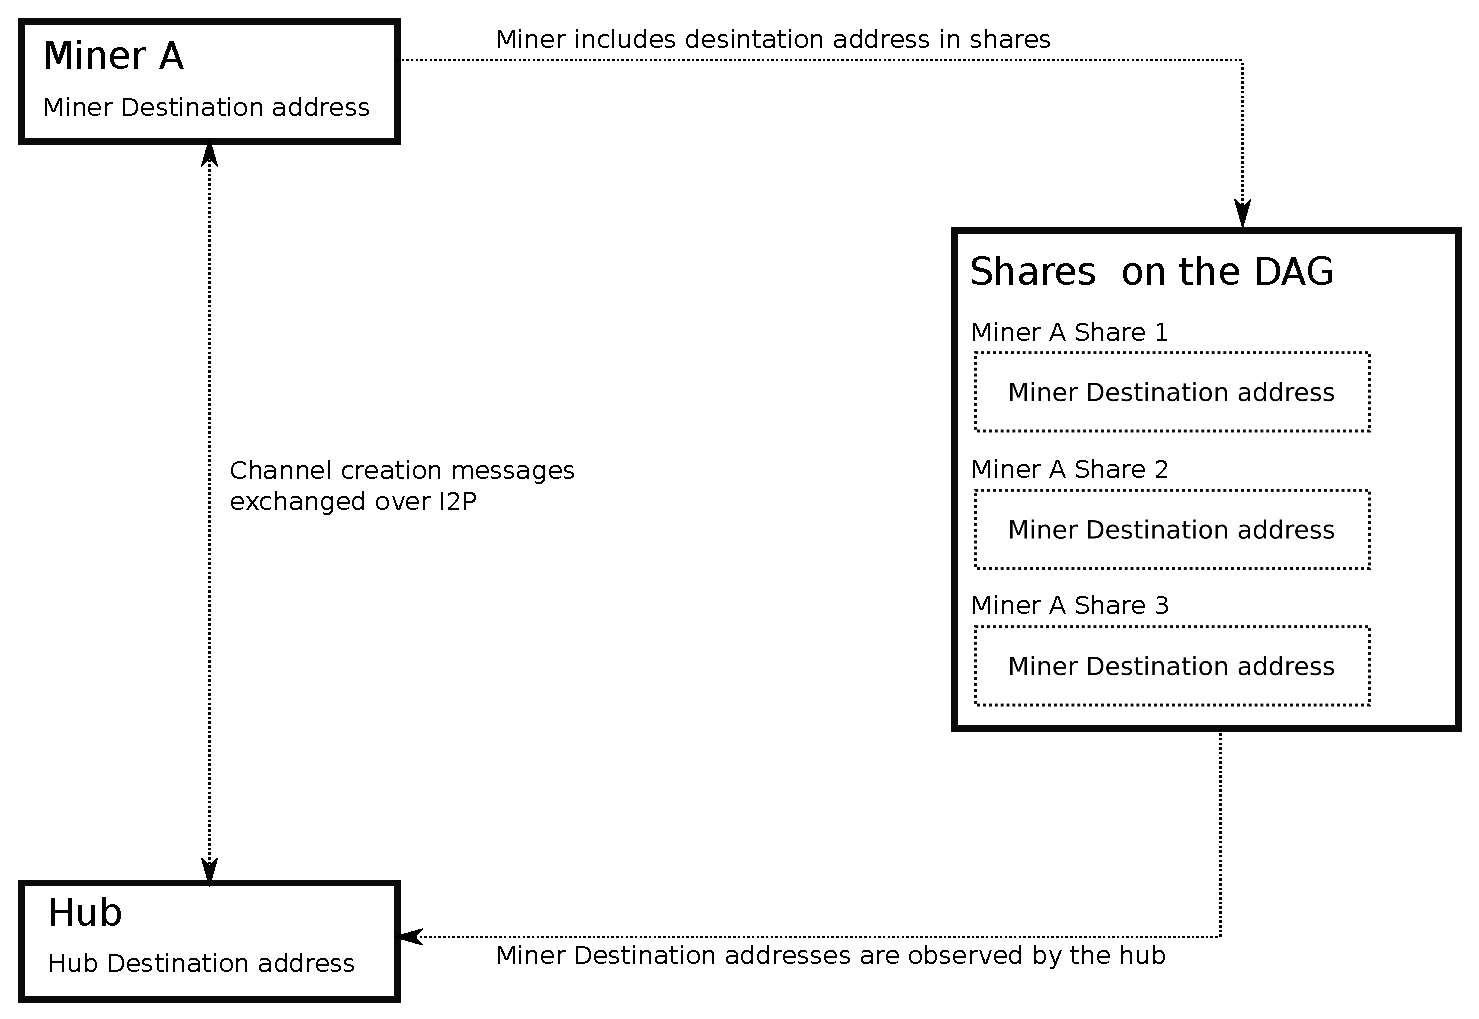
\includegraphics[width=0.8\textwidth]{new-miner-communication.eps}
    \caption{Discovery of miner I2P destination addresses enables
      communication for creating channels.}\label{fig:new-miner-communication}
  \end{center}
\end{figure}

\begin{figure}
  \begin{center}
    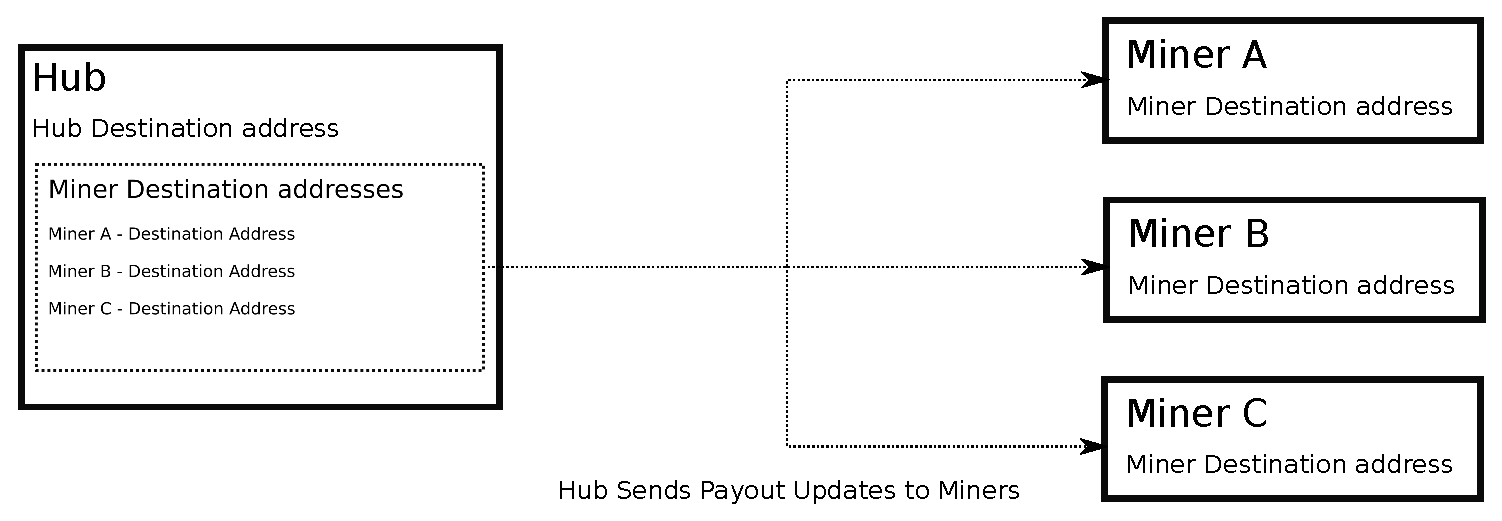
\includegraphics[width=0.8\textwidth]{payout-communication.eps}
    \caption{Hub sends one way updates to miners without revealing its
      destination address.}\label{fig:new-miner-communication}
  \end{center}
\end{figure}

To send payouts as channel state updates, the hub again uses the I2P
destination address of each miner and sends a one way message, with no
reply destination included in the message. This allows the hub to
remain anonymous and makes it relatively hard to DDoS the hub.

\section{Future Work}

The proposal presents an approach to enable decentralised mining for
bitcoin. Apart from the work of describing the various components in
detail, we also want to provide results from simulations, formalised
proofs of rewards schemes and possible extensions to using multiple
hubs.

\subsection{Simulations}

Before we work on implementing they system, our next step is to
simulate p2p mining network using ns-3 [ref] and make informed
decisions about how large a network a single hub can support. The
observations we want to make are how large a p2p network can be
sustained without an increase in work lost by miners. Each hub and p2p
network can grow as long as miners are communicate WORK and SHARES
with each other with bounded latency and can limit their lost
work. With a simulation we want to find out the bounds of these.

\subsection{Specifications}

We want to specify the p2p protocols and the message formats for both
the \textsc{share}s propagation and Channel management networks. By
publishing the specifications separate from the source code, we aim to
receive more feedback from the community.

\subsection{Proofs}

We want to use the model presented in~\cite{incentives-compatible} to
provide proofs for how the rewards distribution is incentives
compatible.

\subsection{Multiple Hubs}

We would like to build further on the multiple hubs construction
described by Belcher once Taproot is activated on bitcoin.

\section{Acknowledgements}

--

\bibliography{proposal} 
\bibliographystyle{acm}

\end{document}
